\documentclass{article}

\usepackage[margin=0.5in]{geometry}
\usepackage{multicol}
\usepackage{amsthm}
\usepackage{amsmath}
\usepackage{tikz}

\theoremstyle{definition}
\newtheorem*{solution}{Solution}
\title{Plane Geometry Set B}
\date{}
\author{}

\begin{document}
\maketitle

\begin{multicols}{2}
    \begin{enumerate}
        \item Points $A$, $B$, $Q$, $D$, and $C$ lie on the circle shown and the measures of arcs $\stackrel{\mbox{\large$\frown$}}{BQ}$ and $\stackrel{\mbox{\large$\frown$}}{QD}$ are $42^{\circ}$ and $38^{\circ}$ respectively.
            What is the sum of angles $P$ and $Q$?
            \begin{center}
                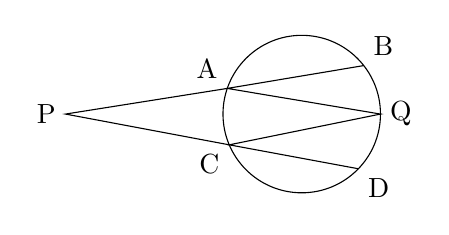
\begin{tikzpicture}
                    \draw (0,0) circle (1cm);
                    \foreach \name /\position /\angle /\radius in {A/{above left}/161/1, B/{above right}/38/1, C/{below left}/203/1, D/{below right}/316/1, P/{left}/180/3, Q/{right}/0/1}
                        \coordinate[label= \position:\name] (\name) at (\angle:\radius);
                    \draw (B) -- (A) -- (Q) -- (C) -- (D);
                    \draw (A) -- (P) -- (C);
                \end{tikzpicture}
            \end{center}
            \begin{solution}
                As the angle formed by two secants, $\angle P = \frac{\stackrel{\mbox{\large$\frown$}}{BD} - \stackrel{\mbox{\large$\frown$}}{AC}}{2}$.
                As an inscribed angle, $\angle Q = \frac{\stackrel{\mbox{\large$\frown$}}{AC}}{2}$.
                Thus, $\angle P + \angle Q = \frac{\stackrel{\mbox{\large$\frown$}}{BD}}{2} = \frac{\stackrel{\mbox{\large$\frown$}}{BQ} + \stackrel{\mbox{\large$\frown$}}{QD}}{2} = \frac{42^{\circ} + 38^{\circ}}{2} = 40^{\circ}$.
            \end{solution}
        \item Kent draws a regular hexagon of side length $4$ cm and then draws a semicircle outward along each side.
            The total area enclosed by Kent's drawing can be expressed in simplest radical form, in terms of $\pi$, as $(a \cdot \sqrt{b} + c\pi)$.
            What is the value of $\frac{a}{b} + c$?
            \begin{solution}
                Kent's drawing is shown here.
                Notice that the hexagon can be divided into six congruent equilateral triangles, making its area six times the area of one of these triangles.
                Each of these triangles has the side length $4$ cm, altitude $2\sqrt{3}$ cm and area $\frac{1}{2} \cdot 4 \cdot 2\sqrt{3} = 4\sqrt{3}$ cm$^{2}$.
                So, the hexagon has area $6 \cdot 4\sqrt{3} = 24\sqrt{3}$ cm$^{2}$.
                Notice also that the six semicircles with diameter $4$ cm and radius $2$ cm have the same area as three circles of the same diameter and radius.
                The area of one such circle is $\pi \cdot 2^{2} = 4\pi$ cm$^{2}$.
                The area of all six semicircles, then, is $3 \cdot 4\pi = 12\pi$ cm$^{2}$.
                Therefore, Kent's entire drawing has area $24\sqrt{3} + 12\pi$ cm$^{2}$, which is in the required form.
                So, $a = 24$, $b = 3$, $c =12$, and $\frac{a}{b} + c = \frac{24}{3} + 12 = 8 + 12 = 20$.
                \begin{center}    
                    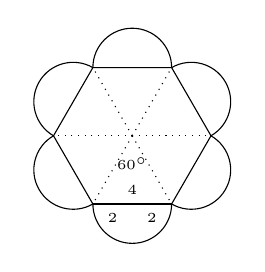
\begin{tikzpicture}
                        \foreach \name /\startangle in {a/0,b/60,c/120,d/180,e/240,f/300}
                            \coordinate (\name) at (\startangle:1); 
                        \coordinate[label=below:{\tiny $60^{\circ}$}] (g) at (270:0.15);
                        \draw (a) -- (b) -- (c) -- (d) -- (e) -- node[midway, above] {\tiny $4$} (f) -- cycle;
                        \draw (e) -- node[near start, below] {\tiny $2$} (f);
                        \draw (e) -- node[near end, below] {\tiny $2$} (f);
                        \foreach \name /\startangle /\endangle in {a/-60/120, b/0/180, c/60/240, d/120/300, e/180/360, f/240/420}
                        {
                            \draw (\name) arc (\startangle:\endangle:0.5);
                            \draw[dotted] (0,0)--(\name);
                        }
                    \end{tikzpicture}
                \end{center}
            \end{solution}
        \item In the figure, if arc $\stackrel{\mbox{\large$\frown$}}{AB} = 60^{\circ}$ and arc $\stackrel{\mbox{\large$\frown$}}{DE} = 40^{\circ}$, then what is $\angle ACD$?
            \begin{center}
                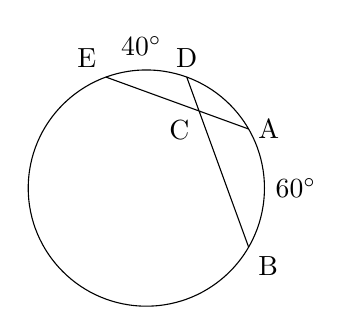
\begin{tikzpicture}
                    \draw (0,0) circle (1.5cm);
                    \coordinate[label=right:A] (A) at (30:1.5);
                    \coordinate[label=below right:B] (B) at (330:1.5);
                    \coordinate[label=above:D] (D) at (70:1.5);
                    \coordinate[label=above left:E] (E) at (110:1.5);
                    \draw (A) -- (E) (B) -- (D);
                    \coordinate[label=below left:C] (C) at (intersection of A--E and B--D);
                    \draw (92:1.8) node {$40^{\circ}$};
                    \draw (360:1.9) node {$60^{\circ}$};
                \end{tikzpicture}
            \end{center}
            \begin{solution}
                Since $\angle ABC$ is one-half the sum of arc $\stackrel{\mbox{\large$\frown$}}{AB}$ and arc $\stackrel{\mbox{\large$\frown$}}{DE}$, we have $\angle ACB = 50^{\circ}$.
                Since $\angle ACB + \angle AC = 180^{\circ}$, we find that $\angle ACD = 130^{\circ}$.
            \end{solution}
        \item The incircle of a triangle is a circle tangent to all three sides of the triangle, as shown in this example.
            What is the radius of the incircle of a right triangle with side lengths of $12$, $35$ and $37$ mm?
            \begin{center}
                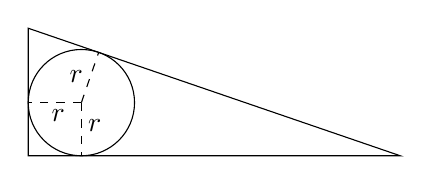
\begin{tikzpicture}
                    \draw (0,0) -- (0, 16.2mm) -- (47.25mm, 0) -- cycle;
                    \draw (6.75mm, 6.75mm) circle (6.75mm);
                    \begin{scope}[shift={(6.75mm,6.75mm)}]
                        \foreach \lineangle /\labelangle in {71/101,180/210,270/300}
                        {
                            \draw [dashed] (0,0) -- (\lineangle:6.75mm);
                            \draw (\labelangle:3.375mm) node {$r$};
                        }
                    \end{scope}
                \end{tikzpicture}
            \end{center}
            \begin{solution}
                A right triangle with an incircle and three radii, each drawn perpendicular to a side of the triangle contains two kites (one at each acute angle), as well as a square of side length $r$ (at the right angle).
                The sum of the lengths of the legs is greater than the length of the hypotenuse by an amount equal to exactly two radii!
                The radius of the incircle, then, is $r = \frac{1}{2} (12 + 35 - 37) = \frac{1}{2} \cdot 10 = 5$ mm.
            \end{solution}
        \item Convex quadrilateral $WXYZ$ is inscribed in a circle.
            If m$\angle XYZ = 54^{\circ}$, what is the degree measure of $XWZ$?
            \begin{solution}
                A quadrilateral that is inscribed in a circle is called cyclic.
                In a cyclic quadrilateral, opposite angles are supplementary.
                So, the measure of $XWZ$ is $180 - 52 = 126^{\circ}$.
            \end{solution}
    \end{enumerate}
\end{multicols}
\end{document}